% !TEX root = Kreisfahrt.tex
\begin{figure}
    \centering
    \includegraphics[width=.9\textwidth]{Abbildungen/Roboter}
    \caption{Der verwendete Roboter mit montiertem Knickarm.}
\end{figure}
\newpage

\section{Einleitung}
Der Mecanum-Roboter ist ein omnidirektionales Fahrzeug. Er kann ohne Lenkung aus jeder Position in eine beliebige Richtung fahren und sich auf der Stelle drehen.
Grund dafür sind die verwendeten Allseitenräder -- Mecanum-Räder -- auf deren Umlauffläche 15 weitere tonnenförmige Hilfsräder angebracht sind.

Ziel ist es, drei Kreisfahrten auf einem Viertelkreis mit dem Durchmesser $4000~mm$ zu realisieren.
Dazu wird zuerst ein mathematisches Modell zur Beschreibung der einzelnen Bewegungen der Räder aufgestellt und dieses anschließend auf einem Mikrocontroller implementiert.

\begin{description}
    \begin{figure}[H]
        \centering
        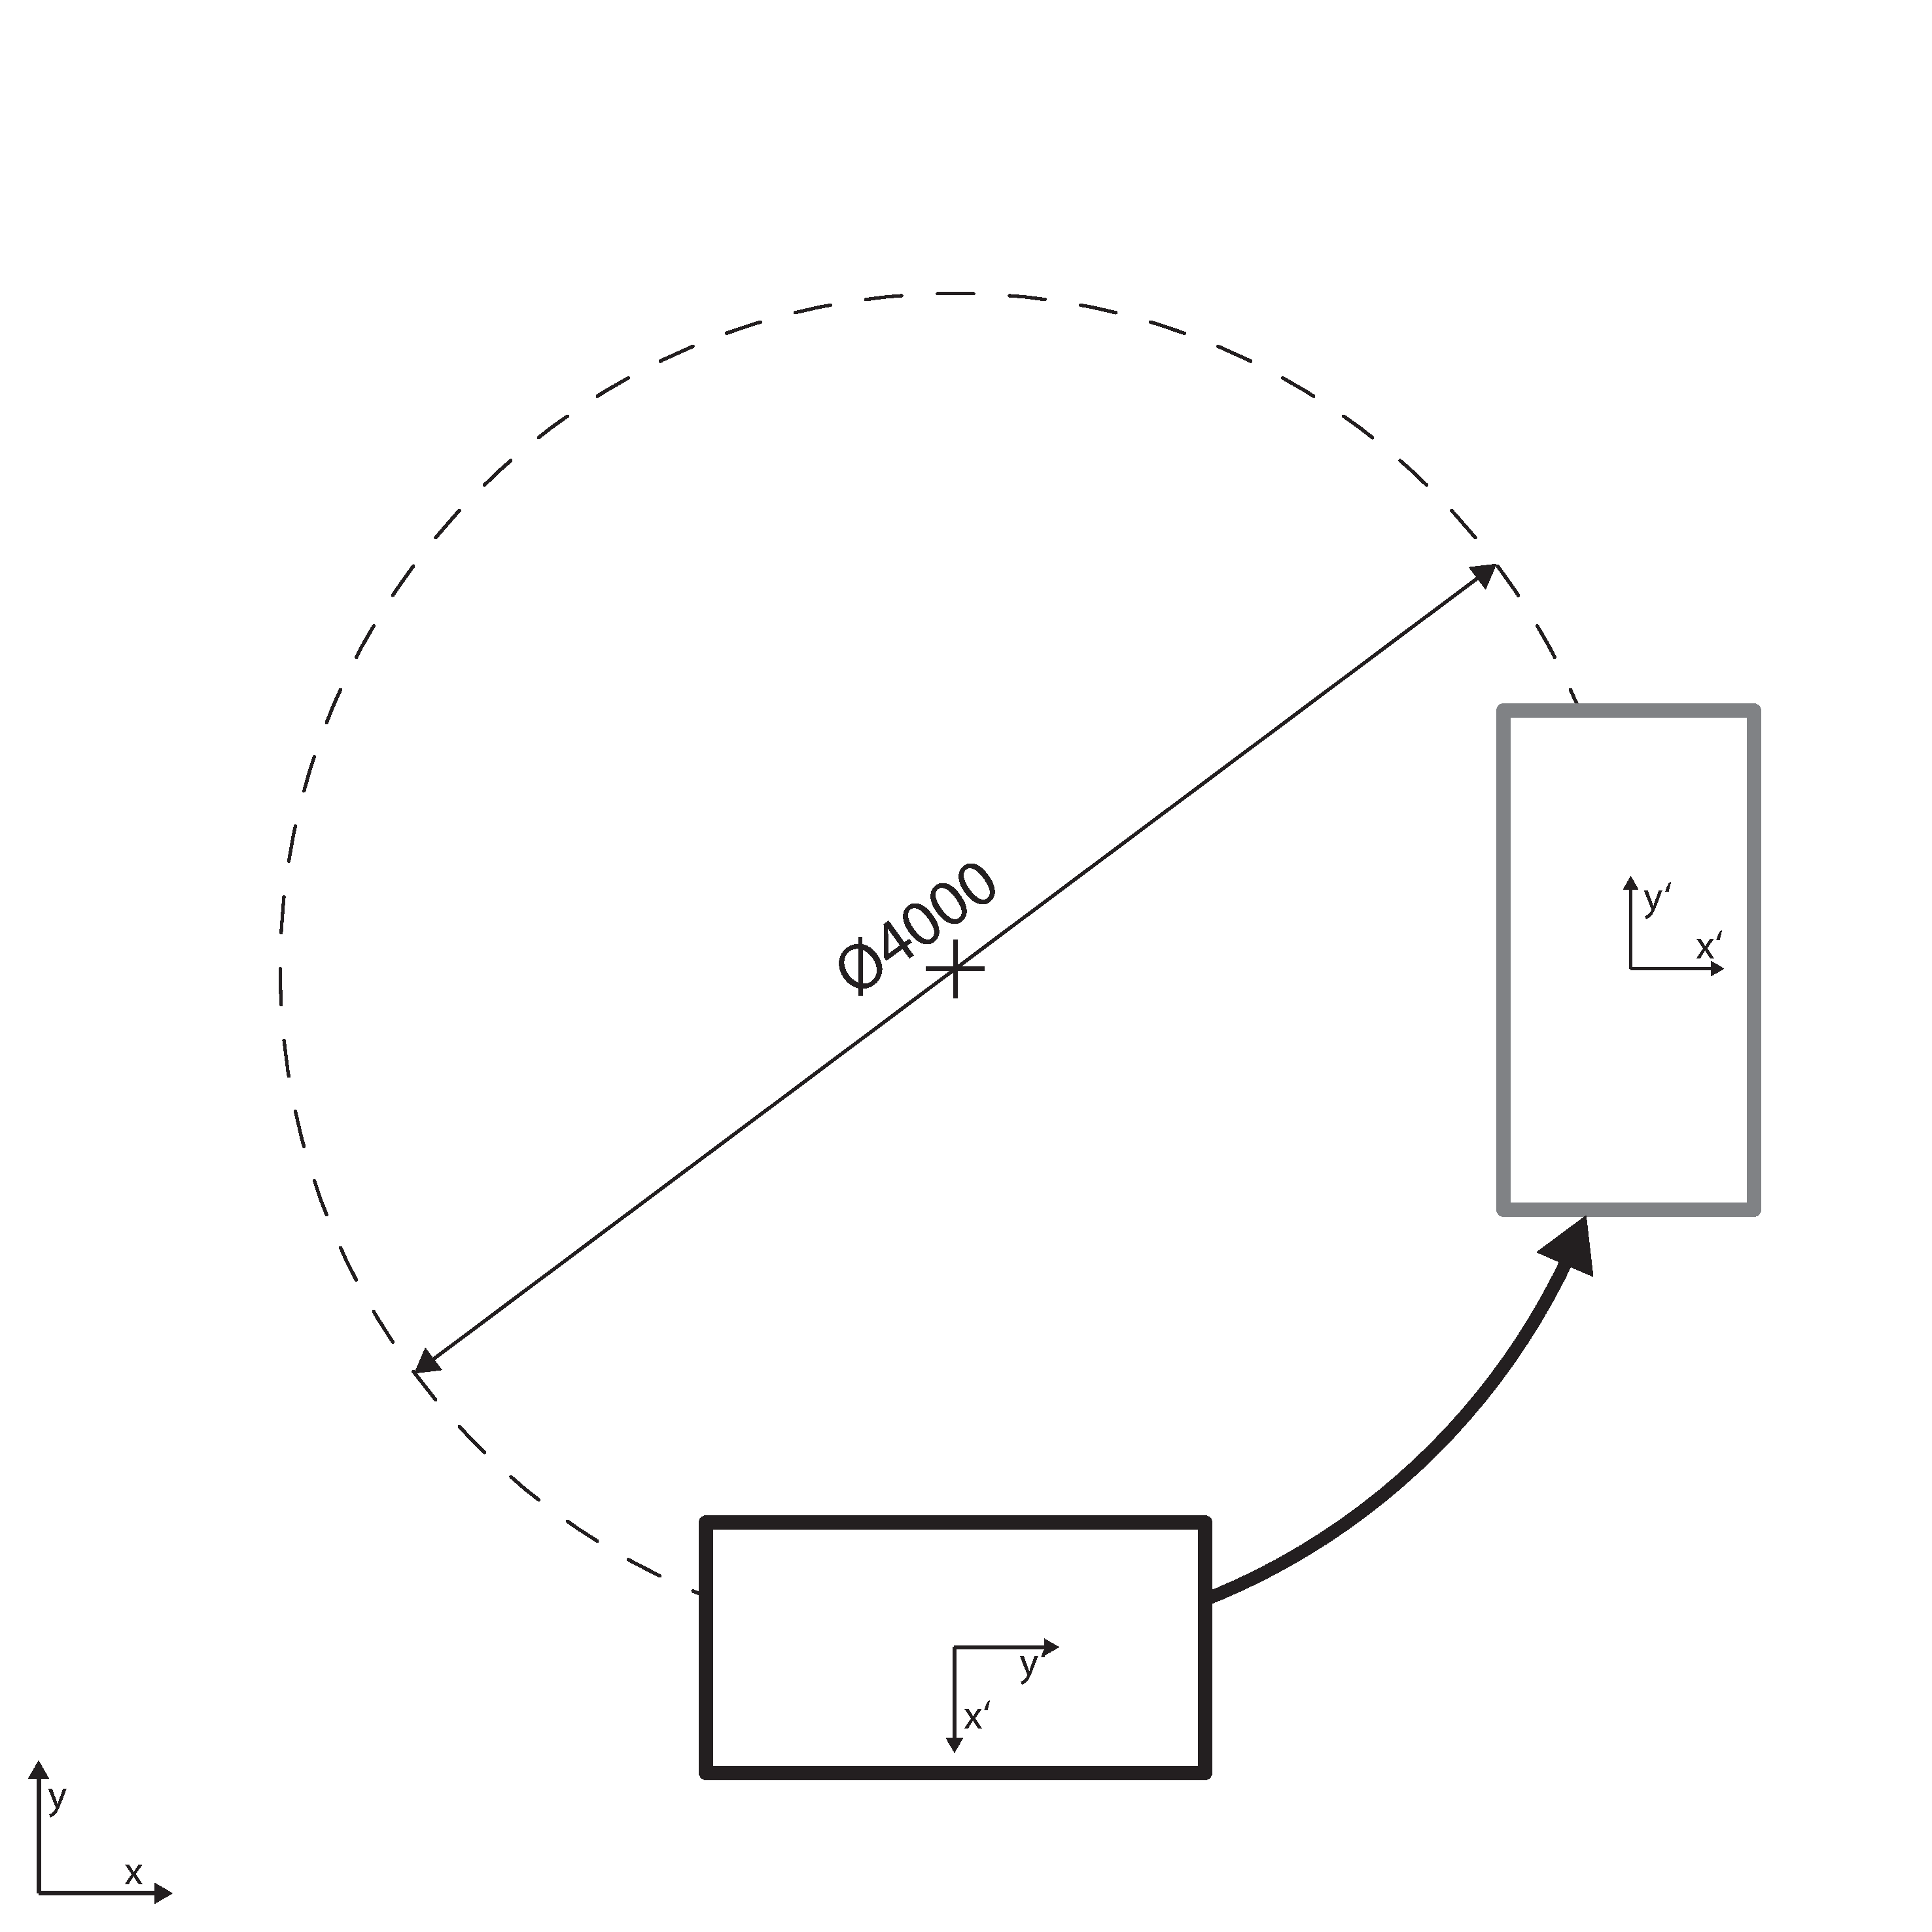
\includegraphics[width=.6\textwidth]{Abbildungen/Viertelkreis-vorwaerts}
        \caption{Kreisfahrt vorwärts}
        \label{fig:kreis-vorwaerts}
    \end{figure}
    \item[Aufgabe 1:]
    Der Mecanum-Roboter fährt einen normalen Viertelkreis. Das Koordinatensystem des Roboters dreht sich dabei während der Kreisfahrt mit, $y'$ ist Tangente des gefahrenen Kreises.

    \begin{figure}[H]
        \centering
        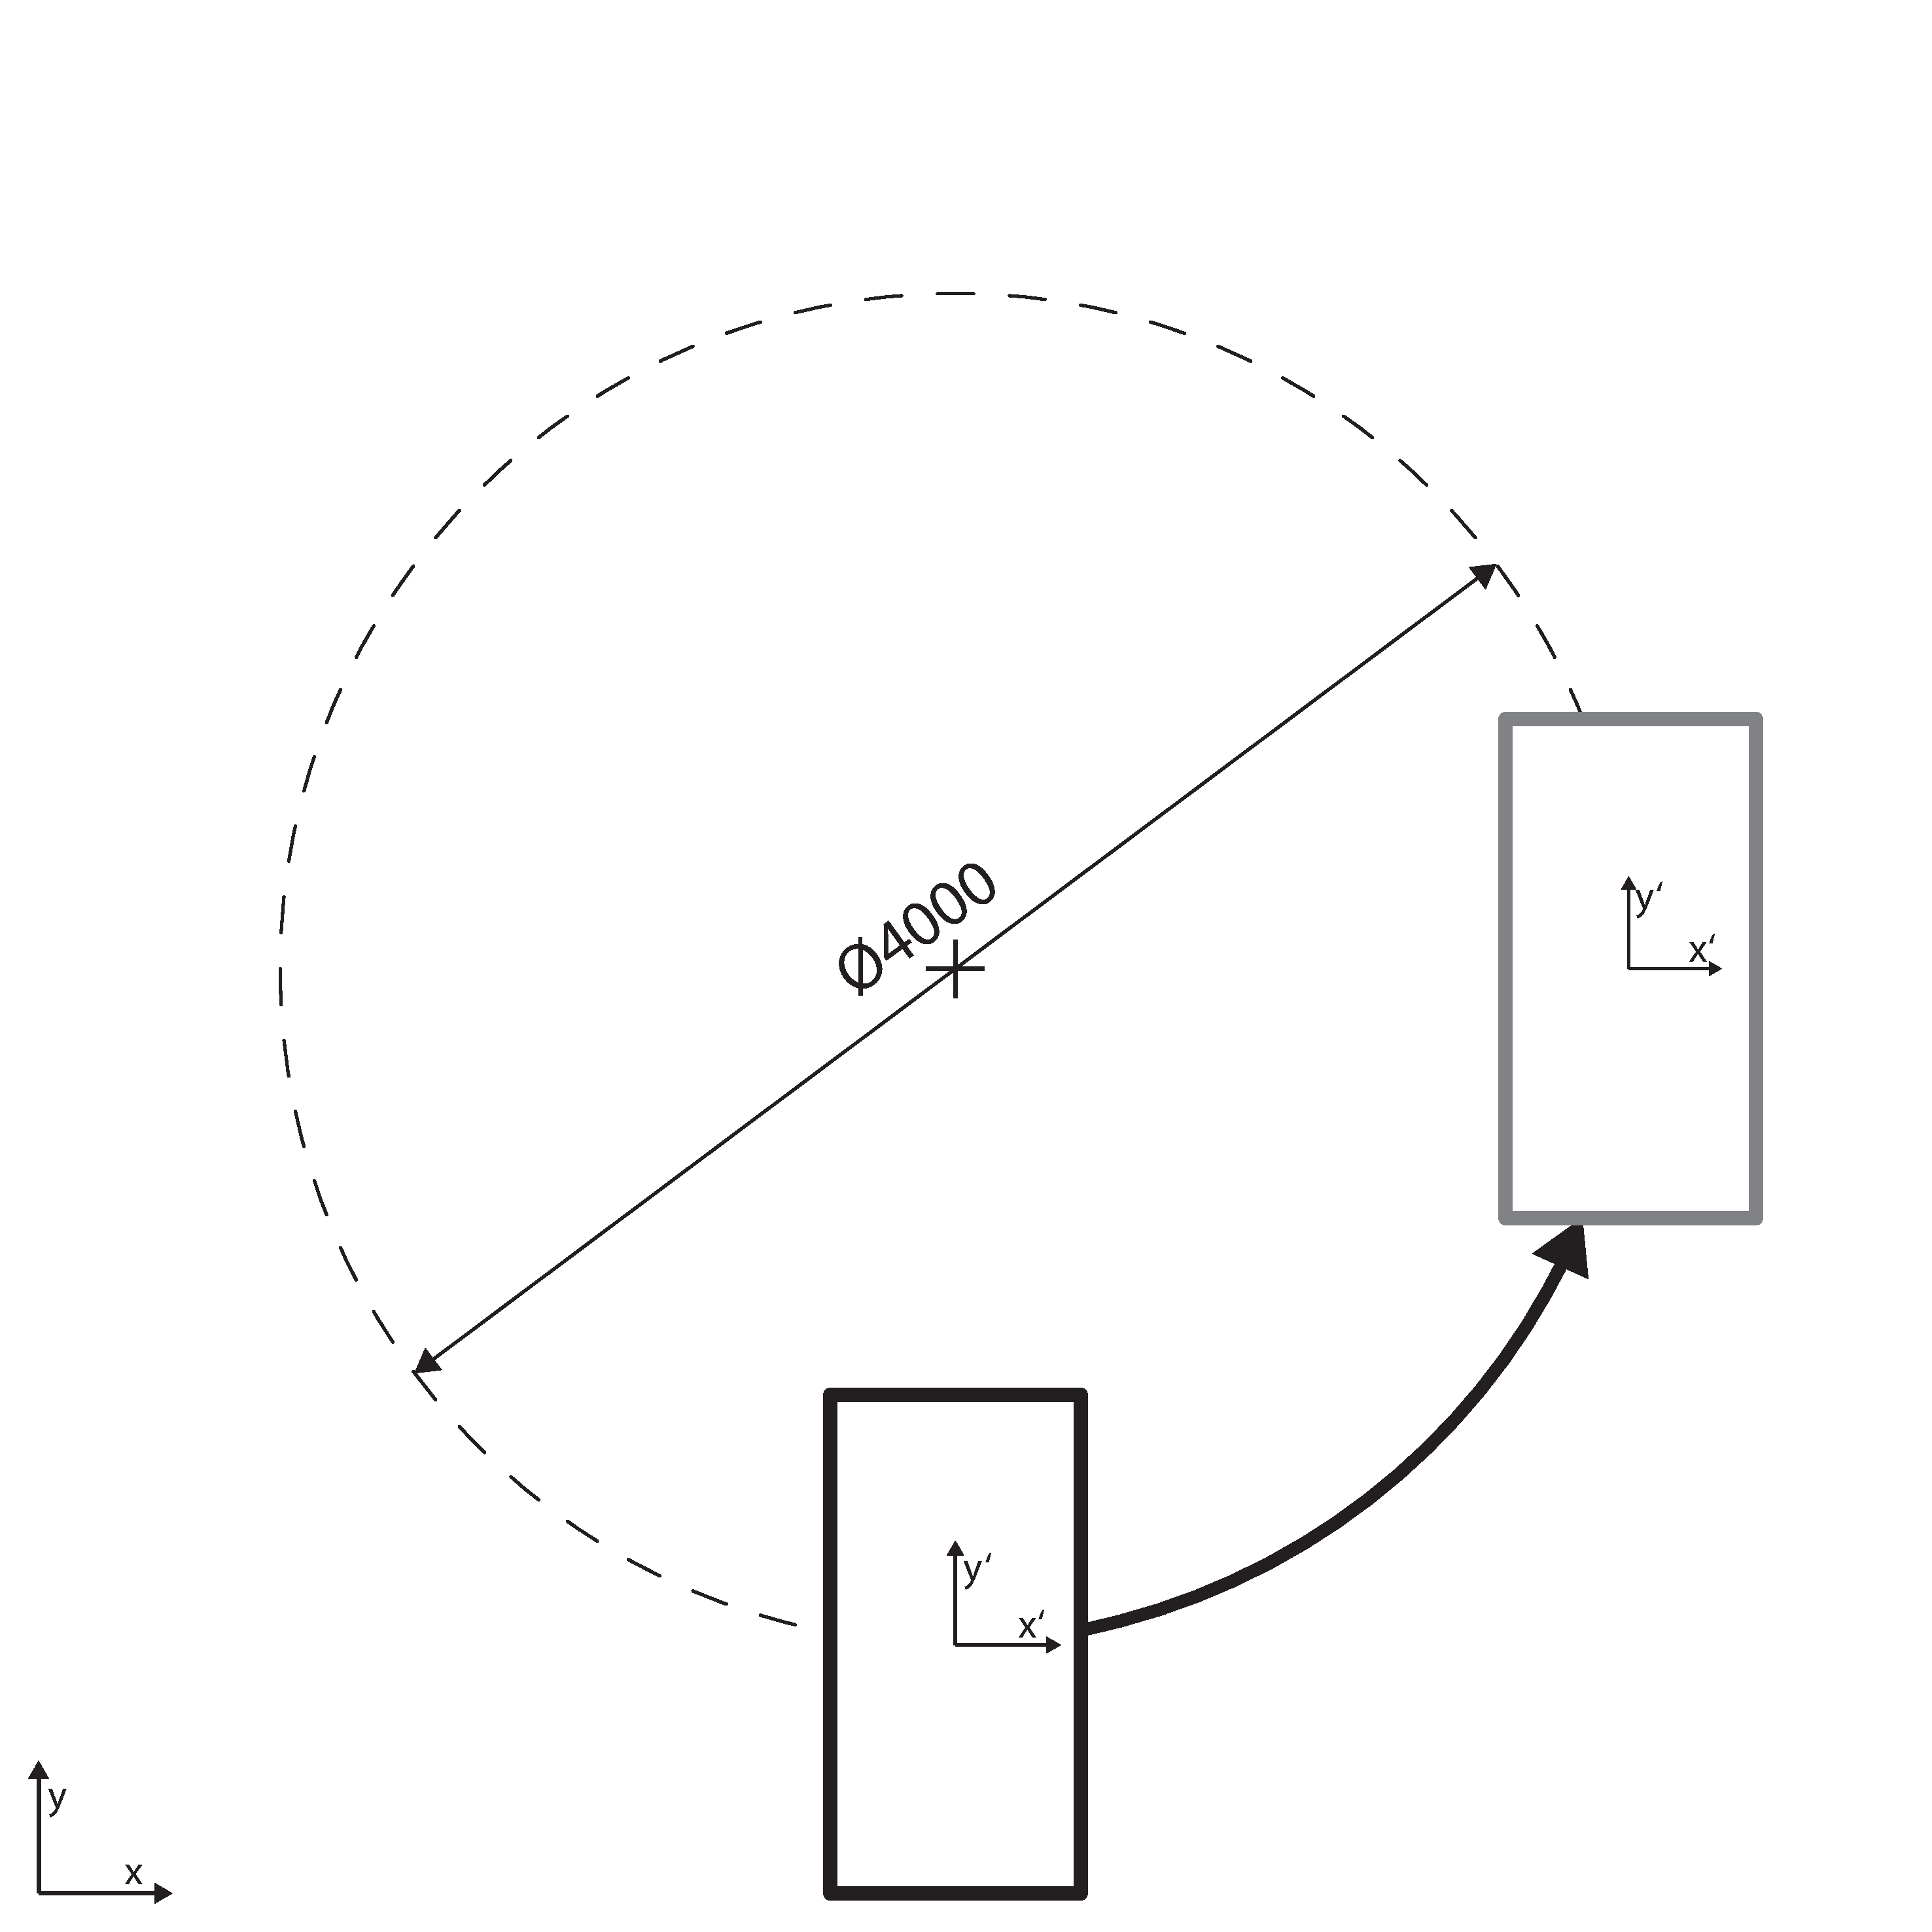
\includegraphics[width=.6\textwidth]{Abbildungen/Viertelkreis-translatorisch}
        \caption{Translatorische Kreisfahrt}
        \label{fig:kreis-translatorisch}
    \end{figure}
    \item[Aufgabe 2:]
    Das Koordinatensystem des Roboters ist stets parallel zu den Raumkoordinaten, während die Bewegung des Robotermittelpunkts im Raum einen Kreis beschreibt.

    \begin{figure}[H]
        \centering
        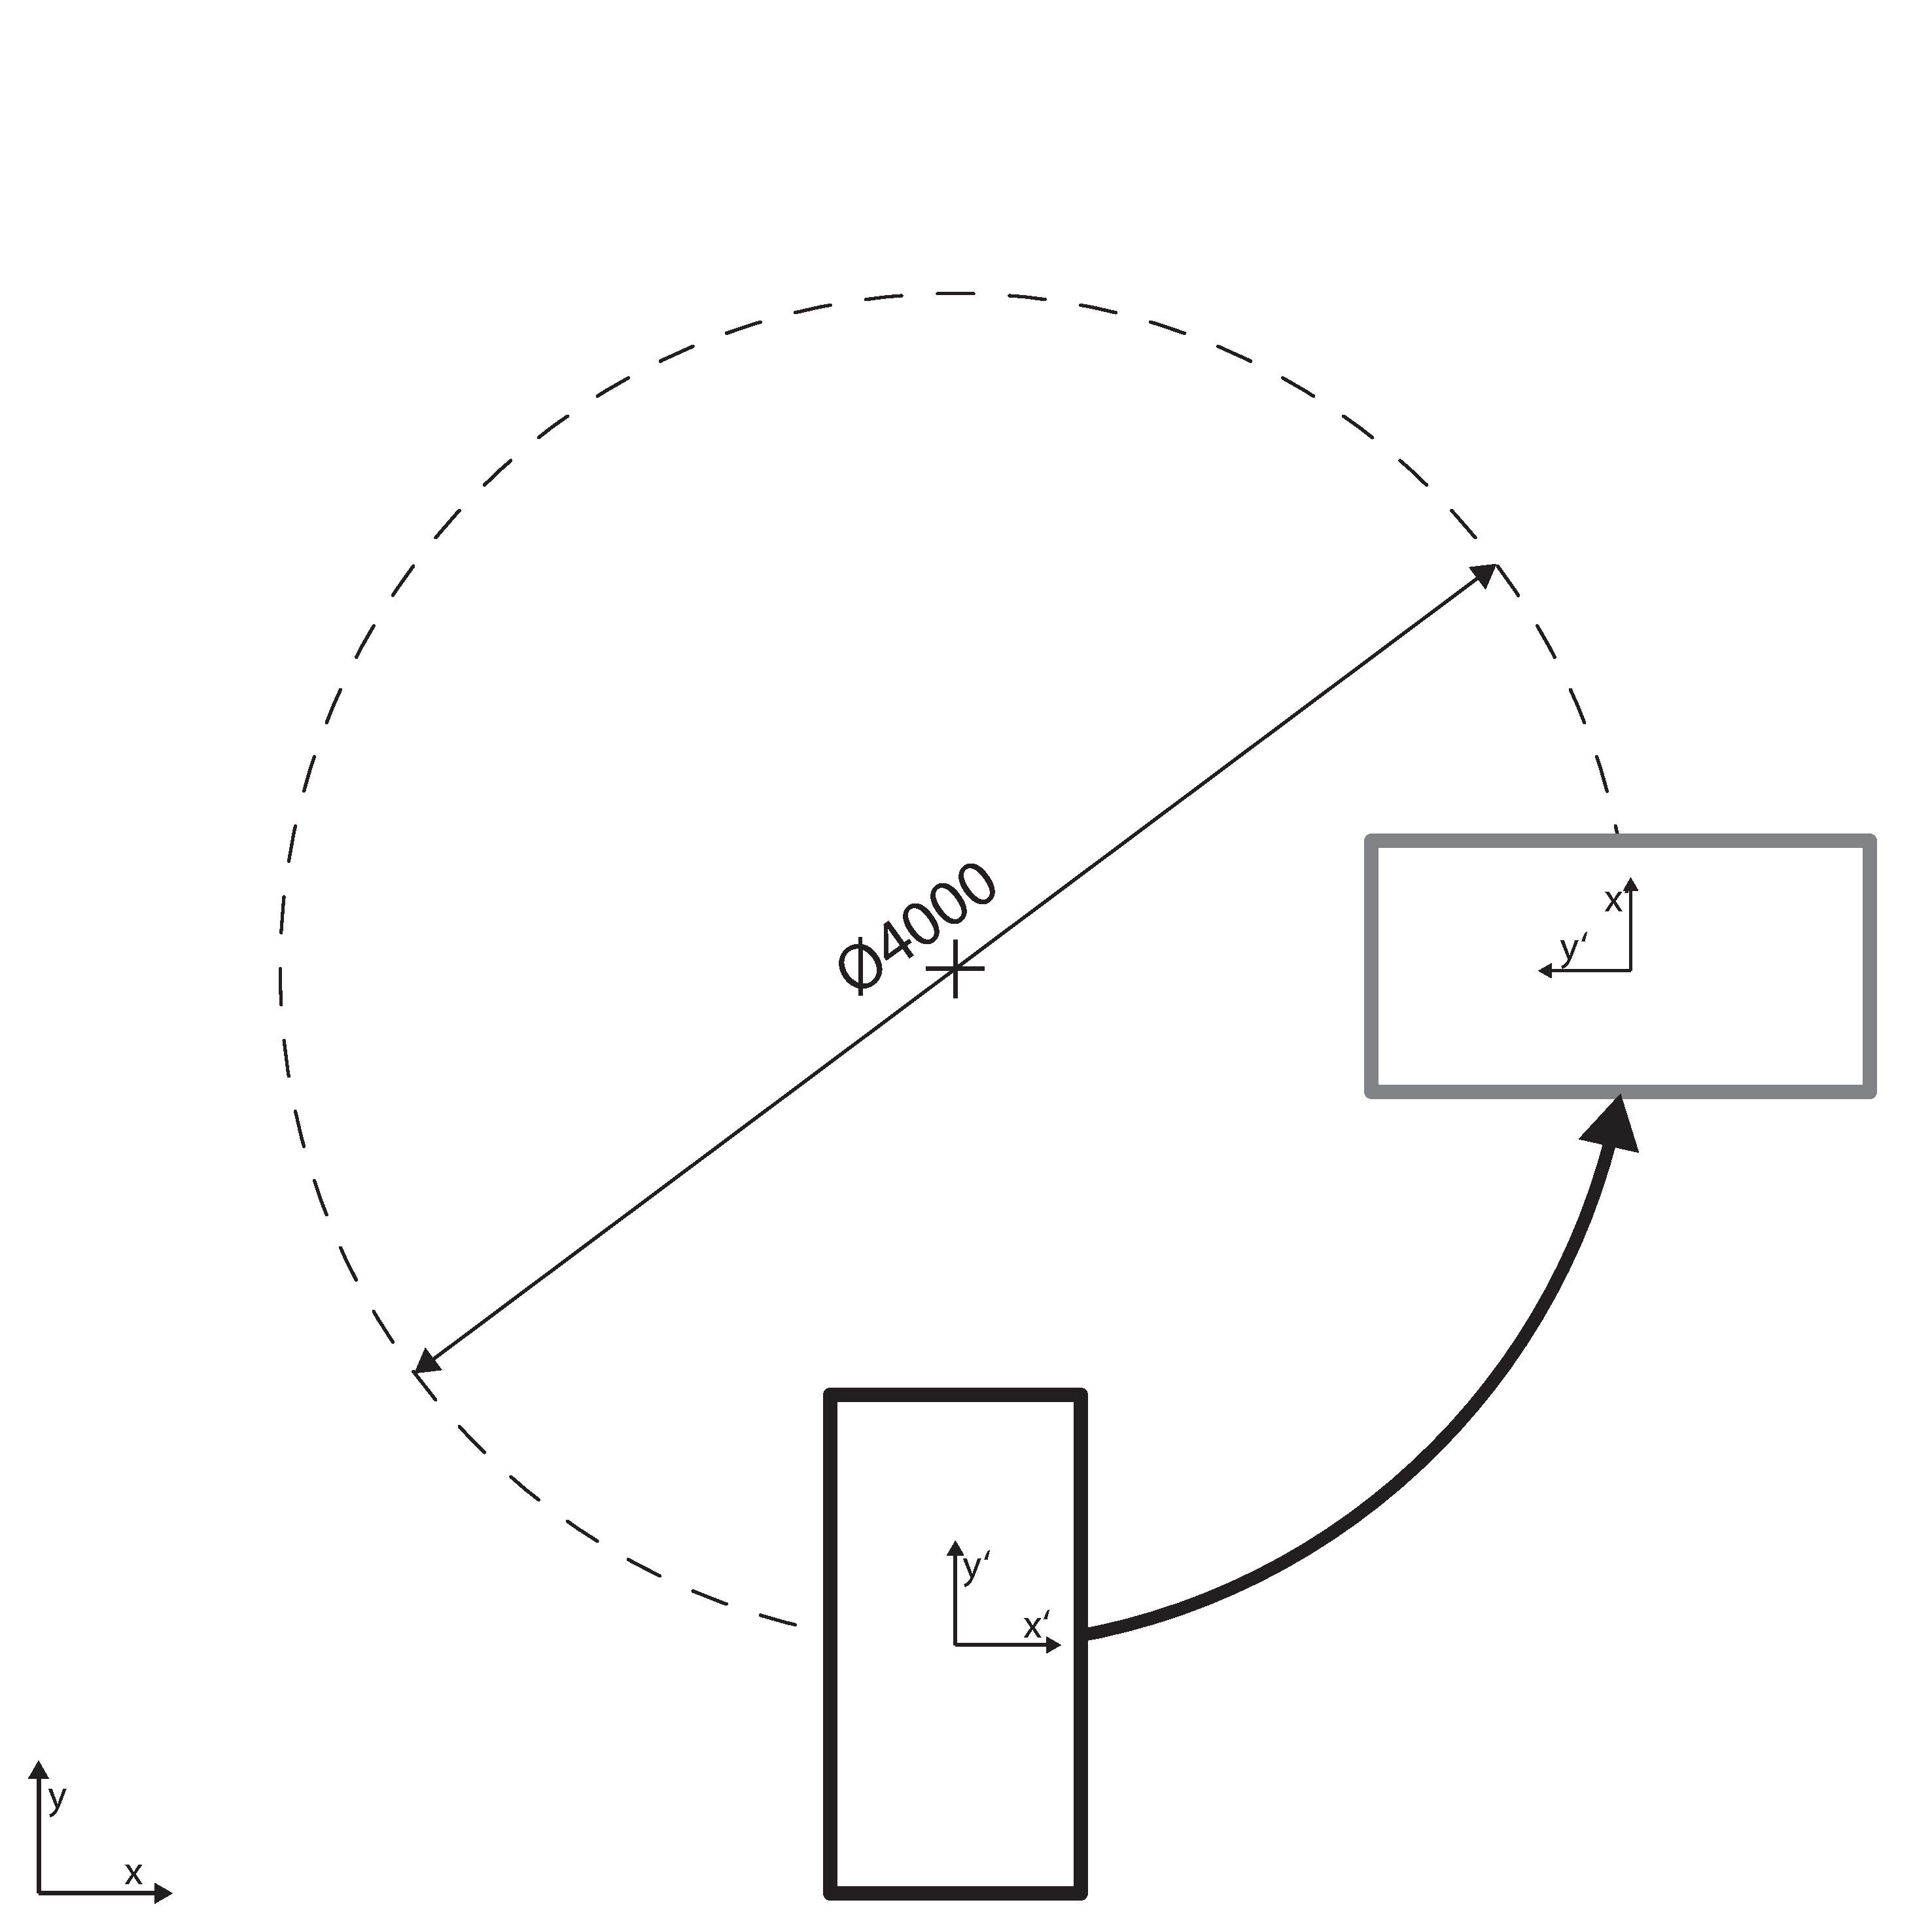
\includegraphics[width=.6\textwidth]{Abbildungen/Viertelkreis-seitwaerts}
        \caption{Kreisfahrt seitlich}
        \label{fig:kreis-seitwaerts}
    \end{figure}
    \item[Aufgabe 3:]
    Das Koordinatensystem des Roboters gegenüber Abbildung~\ref{fig:kreis-vorwaerts} um $90^\circ$ gedreht. $x'$ ist Tangente des gefahrenen Kreises.
\end{description}
